% =====================================================================
% Section 4 of Maximus's notes: Lines
% 4.1 equations (+ practice), 4.2 foot, 4.3 reflection of a point,
% 4.4 shortest distance, 4.5 relationship (+ intersection),
% 4.6 angle, 4.7 reflection of a line about a line.
% Note: page 15 of his notes (4.6, 4.7) has no handwritten working in
% the COMPLETED copy; Example 13.4.13 is solved by his method in 4.2-4.3.
% =====================================================================
\clearpage
\section{Lines}
% =====================================================================
\subsection{Equations of Lines}
% ---------------------------------------------------------------------
A line is fixed by \textbf{one point on it} and \textbf{one direction}. Every equation of a line is a way of writing those two things down.

\begin{definition}{Vector form of a line}
The vector equation of a line is
\[
\mathbf{r} = \mathbf{a} + \lambda\mathbf{b}, \qquad \lambda\in\RR,
\]
where $\mathbf{a}$ is the position vector of \emph{any} point on the line and $\mathbf{b}$ is the \textbf{direction} of the line.
\end{definition}
Each value of $\lambda$ gives one point: $\mathbf{r}$ is the position vector of a general point on the line. Reading the three rows one at a time gives the \textbf{parametric form} $x = a_1 + \lambda b_1$, \ $y = a_2 + \lambda b_2$, \ $z = a_3 + \lambda b_3$.

\begin{definition}{Cartesian form of a line}
Make $\lambda$ the subject of each parametric equation and equate:
\[
\dfrac{x-a_1}{b_1} = \dfrac{y-a_2}{b_2} = \dfrac{z-a_3}{b_3}\ \ (=\lambda).
\]
\end{definition}

\begin{center}
\begin{tikzpicture}[x={(-0.45cm,-0.38cm)}, y={(0.9cm,0cm)}, z={(0cm,0.85cm)}, >=Stealth, scale=0.62]
  \place{A}{1}{2}{-1}
  \place{B}{0}{-2}{1}
  \place{L0}{-1}{-6}{3}
  \place{L1}{2.5}{8}{-4}
  \draw[varr, black!40] (0,0,0) -- (3,0,0) node[left] {$x$};
  \draw[varr, black!40] (0,0,0) -- (0,4,0) node[right] {$y$};
  \draw[varr, black!40] (0,0,0) -- (0,0,3) node[above] {$z$};
  \node[black!50, above left] at (0,0,0) {$O$};
  \draw[blue!70!black, very thick] (L0) -- (L1) node[right] {$l$};
  \draw[varr, teal!55!black, thick] (0,0,0) -- (A) node[midway, left] {$\mathbf{a}$};
  \draw[varr, orange!85!black, very thick] (A) -- (2,6,-3) node[midway, above right] {$\mathbf{b}$};
  \node[pt, label=below left:{$(1,2,-1)$}] at (A) {};
  \node[pt, label=above right:{$(0,-2,1)$}] at (B) {};
\end{tikzpicture}
\end{center}

\begin{caution}
\textbf{The equation of a line is not unique.} Any point on the line can be $\mathbf{a}$, and any non-zero multiple of $\mathbf{b}$ can be the direction. Two correct answers may look different.

\textbf{Edge case: a zero component.} If $b_1 = 0$, you cannot divide by it. That coordinate is constant along the line: write $x = a_1$ separately, and equate the other two fractions.
\end{caution}

% EXAMPLE: from Maximus's notes, 4.1.3 Practice Problems for Equation of Lines
\begin{example}[label=ex:4.1]
Find both the vector and Cartesian equations of the line that passes through
\begin{enumerate}[(a)]
  \item $(1,2,-1)$ and $(0,-2,1)$,
  \item the origin, and is parallel to the vector $3\mathbf{i} + \mathbf{j} - \mathbf{k}$,
  \item $(1,0,1)$, and is perpendicular to both $-\mathbf{i} + \mathbf{j} + 2\mathbf{k}$ and $4\mathbf{i} + \mathbf{j} + 2\mathbf{k}$.
\end{enumerate}
\end{example}
\solution{
(a)\quad Direction $\col{0}{-2}{1} - \col{1}{2}{-1} = \col{-1}{-4}{2}$, or more simply $\col{1}{4}{-2}$.
\[
\mathbf{r} = \ans{ex1341a}{\col{1}{2}{-1}} + \lambda\ans{ex1341ad}{\col{1}{4}{-2}},\ \lambda\in\RR; \qquad
x - 1 = \dfrac{y-2}{4} = \dfrac{z+1}{-2}.
\]
(b)\quad The origin is on the line, so $\mathbf{a} = \mathbf{0}$:
\[
\mathbf{r} = \mu\ans{ex1341bd}{\col{3}{1}{-1}},\ \mu\in\RR; \qquad
\dfrac{x}{3} = y = -z.
\]
(c)\quad A direction perpendicular to both vectors is their vector product:
\[
\col{-1}{1}{2}\times\col{4}{1}{2} = \col{2-2}{-(-2-8)}{-1-4} = \col{0}{10}{-5} = 5\col{0}{2}{-1}.
\]
\[
\mathbf{r} = \ans{ex1341c}{\col{1}{0}{1}} + \alpha\ans{ex1341cd}{\col{0}{2}{-1}},\ \alpha\in\RR; \qquad
\dfrac{y}{2} = \dfrac{z-1}{-1},\ \ x = 1.
\]
}

\begin{mistake}
\textbf{Common mistake:} losing the sign of a negative component in the Cartesian form. For $\mathbf{r} = \mu(3\mathbf{i}+\mathbf{j}-\mathbf{k})$:
\begin{align*}
\dfrac{x}{3} = \dfrac{y}{1} = \dfrac{z}{1}, \ \text{i.e. } \dfrac{x}{3} = y = z & & \wrong \\
\dfrac{x}{3} = \dfrac{y}{1} = \dfrac{z}{-1}, \ \text{i.e. } \dfrac{x}{3} = y = -z & & \cmark
\end{align*}
Check one point: $\mu = 1$ gives $(3,1,-1)$, and $-z = 1 = y$.
\end{mistake}

% EXAMPLE: new, for his note "know how to tell if a point lies on a given line"
\begin{example}[label=ex:4.2]
Determine whether the points $P(3,10,-5)$ and $Q(2,5,-3)$ lie on the line $\mathbf{r} = \col{1}{2}{-1} + \lambda\col{1}{4}{-2}$.
\end{example}
\solution{
Solve for $\lambda$ in each row; the point is on the line only if \textbf{all three} give the same $\lambda$.

$P$: \ $1+\lambda = 3$, \ $2+4\lambda = 10$, \ $-1-2\lambda = -5$ all give $\lambda = \ans{ex1342}{2}$. So $P$ lies on the line.

$Q$: \ $1+\lambda = 2$ gives $\lambda = 1$, but $2+4\lambda = 5$ gives $\lambda = \dfrac{3}{4}$. So $Q$ does not lie on the line.
}

% ---------------------------------------------------------------------
\clearpage
\subsection{Foot of Perpendicular (Point to Line)}
% ---------------------------------------------------------------------
Given a point $A$ and a line $l$, the \textbf{foot of the perpendicular} from $A$ to $l$ is the point $F$ on $l$ with $AF\perp l$. It is the point of $l$ closest to $A$.

\begin{definition}{{Method: foot of perpendicular from $A$ to $l:\ \mathbf{r} = \mathbf{a} + \lambda\mathbf{b}$}}
\begin{enumerate}
  \item $F$ lies on $l$, so $\overrightarrow{OF} = \mathbf{a} + \lambda\mathbf{b}$ for some value of $\lambda$.
  \item Write $\overrightarrow{AF} = \overrightarrow{OF} - \overrightarrow{OA}$, in terms of $\lambda$.
  \item $\overrightarrow{AF}\perp l$, so $\overrightarrow{AF}\cdot\mathbf{b} = 0$. Solve for $\lambda$.
  \item Substitute $\lambda$ back into $\overrightarrow{OF}$.
\end{enumerate}
\end{definition}

\begin{center}
\begin{tikzpicture}[x={(-0.45cm,-0.38cm)}, y={(0.9cm,0cm)}, z={(0cm,0.85cm)}, >=Stealth, scale=0.7]
  \place{A}{3}{-2}{-1}
  \place{F}{4}{2}{2}
  \place{L0}{-2}{2}{4}
  \place{L1}{8.5}{2}{0.5}
  \place{P1}{1}{2}{3}
  \draw[blue!70!black, very thick] (L1) -- (L0) node[right] {$l_1$};
  \draw[varr, orange!85!black, very thick] (P1) -- (F) node[midway, above left] {$\mathbf{b}$};
  \draw[red!70!black, very thick, dashed] (A) -- (F);
  \node[pt, label=left:{$A(3,-2,-1)$}] at (A) {};
  \node[pt, label=right:{$F(4,2,2)$}] at (F) {};
  \node[pt, label=right:{$B(1,2,3)$}] at (P1) {};
\end{tikzpicture}
\end{center}
The picture is Example \ref{ex:4.3}: the dashed segment $AF$ meets $l_1$ at a right angle (in space; a flat drawing cannot show every right angle as one).

% EXAMPLE: from Maximus's notes, 4.2 Example 1
\begin{example}[label=ex:4.3]
Find the foot of perpendicular of the point $A(3,-2,-1)$ on the line
\[
l_1:\ \mathbf{r} = \col{1}{2}{3} + \lambda\col{3}{0}{-1},\ \lambda\in\RR.
\]
\end{example}
\solution{
Let $F$ be the foot. Since $F$ lies on $l_1$, \ $\overrightarrow{OF} = \col{1+3\lambda}{2}{3-\lambda}$ for some $\lambda$, and
\[
\overrightarrow{AF} = \col{1+3\lambda}{2}{3-\lambda} - \col{3}{-2}{-1} = \col{3\lambda-2}{4}{4-\lambda}.
\]
$\overrightarrow{AF}\perp l_1$: \quad $\col{3\lambda-2}{4}{4-\lambda}\cdot\col{3}{0}{-1} = 9\lambda - 6 - 4 + \lambda = 10\lambda - 10 = 0$, so $\lambda = 1$.

$\overrightarrow{OF} = \col{4}{2}{2}$: the foot is $\ans{ex1343}{\col{4}{2}{2}}$, i.e.\ $F(4,2,2)$.
}

% EXAMPLE: from Maximus's notes, 4.2 Example 2
\begin{example}[label=ex:4.4]
Find the coordinates of the foot of perpendicular of the point $P(-2,1,1)$ on the line
\[
l_1:\ \mathbf{r} = \col{-4}{1}{0} + \mu\col{0}{1}{-1},\ \mu\in\RR.
\]
\end{example}
\solution{
$\overrightarrow{OF} = \col{-4}{1+\mu}{-\mu}$, so $\overrightarrow{PF} = \col{-4}{1+\mu}{-\mu} - \col{-2}{1}{1} = \col{-2}{\mu}{-\mu-1}$.

$\overrightarrow{PF}\cdot\col{0}{1}{-1} = 0 + \mu + \mu + 1 = 2\mu + 1 = 0$, so $\mu = -\dfrac{1}{2}$.

$\overrightarrow{OF} = \col{-4}{\dfrac{1}{2}}{\dfrac{1}{2}}$: the foot is $\ans{ex1344}{\col{-4}{\dfrac{1}{2}}{\dfrac{1}{2}}}$, i.e.\ $F\!\left(-4,\dfrac{1}{2},\dfrac{1}{2}\right)$.
}

\begin{mistake}
\textbf{Common mistake:} dotting the \emph{position vector} of $F$ with the direction, instead of $\overrightarrow{AF}$. In Example \ref{ex:4.3}:
\begin{align*}
\overrightarrow{OF}\cdot\mathbf{b} = 3(1+3\lambda) - (3-\lambda) = 10\lambda = 0 \ \Rightarrow\ \lambda = 0,\ F(1,2,3) & & \wrong \\
\overrightarrow{AF}\cdot\mathbf{b} = 10\lambda - 10 = 0 \ \Rightarrow\ \lambda = 1,\ F(4,2,2) & & \cmark
\end{align*}
$\overrightarrow{OF}\cdot\mathbf{b} = 0$ finds the foot of the perpendicular from the \emph{origin}, not from $A$.
\end{mistake}

% ---------------------------------------------------------------------
\clearpage
\subsection{Reflection (Point about Line)}
% ---------------------------------------------------------------------
To reflect a point $A$ about a line, first find the foot $F$ (Section \chapnum.4.2). The image $A'$ is on the other side of the line, as far from $F$ as $A$ is, so $F$ is the \textbf{midpoint} of $AA'$.

\begin{definition}{Reflection of a point about a line}
If $F$ is the foot of the perpendicular from $A$ to the line, and $A'$ is the reflection of $A$, then
\[
\overrightarrow{OF} = \dfrac{\overrightarrow{OA} + \overrightarrow{OA'}}{2}
\quad\Longrightarrow\quad
\overrightarrow{OA'} = 2\overrightarrow{OF} - \overrightarrow{OA}.
\]
\end{definition}

\begin{center}
\begin{tikzpicture}[x={(-0.45cm,-0.38cm)}, y={(0.9cm,0cm)}, z={(0cm,0.85cm)}, >=Stealth, scale=0.6]
  \place{A}{3}{-2}{-1}
  \place{F}{4}{2}{2}
  \place{Ap}{5}{6}{5}
  \place{L0}{-2}{2}{4}
  \place{L1}{8.5}{2}{0.5}
  \draw[blue!70!black, very thick] (L1) -- (L0) node[right] {$l_1$};
  \draw[red!70!black, thick, dashed] (A) -- (Ap);
  \node[pt, label=left:{$A(3,-2,-1)$}] at (A) {};
  \node[pt, label=left:{$F(4,2,2)$}] at (F) {};
  \node[pt, label=right:{$A'(5,6,5)$}] at (Ap) {};
\end{tikzpicture}
\end{center}

% EXAMPLE: from Maximus's notes, 4.3 Example 1
\begin{example}[label=ex:4.5]
Find the reflection of the point $A(3,-2,-1)$ about the line $l_1:\ \mathbf{r} = \col{1}{2}{3} + \lambda\col{3}{0}{-1},\ \lambda\in\RR$.
\end{example}
\solution{
From Example \ref{ex:4.3}, the foot is $F(4,2,2)$. Then
\begin{align*}
\overrightarrow{OF} &= \dfrac{\overrightarrow{OA} + \overrightarrow{OA'}}{2}\\
\overrightarrow{OA'} &= 2\overrightarrow{OF} - \overrightarrow{OA}\\
&= 2\col{4}{2}{2} - \col{3}{-2}{-1}\\
&= \ans{ex1345}{\col{5}{6}{5}}
\end{align*}
so $A'(5,6,5)$. Check: $\dfrac{1}{2}\big((3,-2,-1) + (5,6,5)\big) = (4,2,2) = F$.
}

% EXAMPLE: from Maximus's notes, 4.3 Example 2 (typed key P'(6,0,0); his
% handwritten working corrects it to (-6,0,0))
\begin{example}[label=ex:4.6]
Find the reflection of the point $P(-2,1,1)$ about the line $l_1:\ \mathbf{r} = \col{-4}{1}{0} + \mu\col{0}{1}{-1},\ \mu\in\RR$.
\end{example}
\solution{
From Example \ref{ex:4.4}, the foot is $F\!\left(-4,\dfrac{1}{2},\dfrac{1}{2}\right)$. Then
\begin{align*}
\overrightarrow{OF} &= \dfrac{\overrightarrow{OP} + \overrightarrow{OP'}}{2}\\
\overrightarrow{OP'} &= 2\overrightarrow{OF} - \overrightarrow{OP}\\
&= \col{-8}{1}{1} - \col{-2}{1}{1}\\
&= \ans{ex1346}{\col{-6}{0}{0}}
\end{align*}
so $P'(-6,0,0)$.
}

\begin{mistake}
\textbf{Common mistake:} subtracting the wrong way round, $\overrightarrow{OA'} = \overrightarrow{OA} - 2\overrightarrow{OF}$. In Example \ref{ex:4.6}:
\begin{align*}
\overrightarrow{OP'} = \overrightarrow{OP} - 2\overrightarrow{OF} = \col{-2}{1}{1} - \col{-8}{1}{1} = \col{6}{0}{0} & & \wrong \\
\overrightarrow{OP'} = 2\overrightarrow{OF} - \overrightarrow{OP} = \col{-8}{1}{1} - \col{-2}{1}{1} = \col{-6}{0}{0} & & \cmark
\end{align*}
Check the midpoint: $\dfrac{1}{2}\big((-2,1,1) + (6,0,0)\big) = \left(2,\dfrac{1}{2},\dfrac{1}{2}\right)$, which is not $F$. Always check that $F$ is the midpoint.
\end{mistake}

% EXAMPLE: new; the one case where O F . b = 0 is the right equation
\begin{example}[label=ex:4.6b]
Find the reflection of the origin $O$ about the line $l_1:\ \mathbf{r} = \col{1}{2}{3} + \lambda\col{3}{0}{-1}$.
\end{example}
\solution{
Here the point \emph{is} $O$, so $\overrightarrow{OF}\cdot\mathbf{b} = 0$ is the right equation: $3(1+3\lambda) - (3-\lambda) = 10\lambda = 0$, so $\lambda = 0$ and $F(1,2,3)$.
Then $\overrightarrow{OO'} = 2\overrightarrow{OF} - \mathbf{0} = \ans{ex1346b}{\col{2}{4}{6}}$, so $O'(2,4,6)$.
}

\begin{info}
\textbf{Intermediate step.} Every reflection question is a foot-of-perpendicular question first. The same midpoint formula reflects a point about a plane (Section \chapnum.5.3); only the way of finding $F$ changes.
\end{info}

% ---------------------------------------------------------------------
\clearpage
\subsection{Shortest Distance (Point to Line)}
% ---------------------------------------------------------------------
The shortest distance from a point $A$ to a line is the perpendicular distance $AF$. Section \chapnum.3.2 gives it without finding $F$: take \emph{any} point $B$ on the line, and use the vector product.

\begin{definition}{{Shortest distance from $A$ to $l:\ \mathbf{r} = \mathbf{a} + \lambda\mathbf{b}$}}
Let $B$ be any point on $l$ (for example the point with position vector $\mathbf{a}$). Then
\[
\text{Shortest distance} = \left|\overrightarrow{BA}\times\hat{\mathbf{b}}\right| = \dfrac{\left|\overrightarrow{BA}\times\mathbf{b}\right|}{|\mathbf{b}|}.
\]
\end{definition}

\begin{center}
\begin{tikzpicture}[scale=1.0]
  \draw[blue!70!black, very thick] (-0.5,0) -- (7,0) node[right] {$l$};
  \coordinate (B) at (5.2,0);
  \coordinate (A) at (1.6,2.3);
  \coordinate (F) at (1.6,0);
  \draw[varr, teal!55!black, very thick] (B) -- (A) node[midway, above right] {$\overrightarrow{BA}$};
  \draw[red!70!black, thick, dashed] (A) -- (F);
  \draw[red!70!black] (F) ++(0.25,0) -- ++(0,0.25) -- ++(-0.25,0);
  \draw[varr, orange!85!black, very thick] (5.2,0) -- (6.4,0) node[below] {$\mathbf{b}$};
  \node[pt, label=above:{$A$}] at (A) {};
  \node[pt, label=below:{$B$}] at (B) {};
  \node[pt, label=below:{$F$}] at (F) {};
  \node[red!70!black, left] at (1.6,1.1) {$|\overrightarrow{BA}\times\hat{\mathbf{b}}|$};
\end{tikzpicture}
\end{center}

\begin{info}
\textbf{Two routes.} If the foot $F$ is already known (say from an earlier part), the distance is simply $|\overrightarrow{AF}|$. If it is not, finding $F$ just to get a distance is unnecessary and tedious: use the cross product.
\end{info}

% EXAMPLE: from Maximus's notes, 4.4 Example 1
\begin{example}[label=ex:4.7]
Find the shortest distance from the point $A(3,-2,-1)$ to the line $l_1:\ \mathbf{r} = \col{1}{2}{3} + \lambda\col{3}{0}{-1},\ \lambda\in\RR$.
\end{example}
\solution{
Take $B(1,2,3)$ on $l_1$. \ $\overrightarrow{AB} = \col{1}{2}{3} - \col{3}{-2}{-1} = \col{-2}{4}{4}$.
\[
\text{Distance} = \dfrac{\left|\col{-2}{4}{4}\times\col{3}{0}{-1}\right|}{\left|\col{3}{0}{-1}\right|}
= \dfrac{\left|\col{-4}{10}{-12}\right|}{\sqrt{10}}
= \dfrac{\sqrt{260}}{\sqrt{10}} = \ans{ex1347}{\sqrt{26}}\ \text{units}.
\]
($\overrightarrow{AB}$ and $\overrightarrow{BA}$ give the same modulus.) Check with the foot $F(4,2,2)$: $|\overrightarrow{AF}| = \left|\col{1}{4}{3}\right| = \sqrt{26}$.
}

% EXAMPLE: from Maximus's notes, 4.4 Example 2
\begin{example}[label=ex:4.8]
Find the perpendicular distance from the point $P(-2,1,1)$ to the line $l_1:\ \mathbf{r} = \col{-4}{1}{0} + \mu\col{0}{1}{-1},\ \mu\in\RR$.
\end{example}
\solution{
Take $B(-4,1,0)$ on $l_1$. \ $\overrightarrow{BP} = \col{-2}{1}{1} - \col{-4}{1}{0} = \col{2}{0}{1}$.
\[
\text{Length} = \dfrac{\left|\col{2}{0}{1}\times\col{0}{1}{-1}\right|}{\left|\col{0}{1}{-1}\right|}
= \dfrac{\left|\col{-1}{2}{2}\right|}{\sqrt{2}} = \ans{ex1348}{\dfrac{3}{\sqrt{2}}}\ \text{units}.
\]
}

\begin{mistake}
\textbf{Common mistake:} dividing by the wrong length, $|\overrightarrow{BP}|$ instead of $|\mathbf{b}|$.
\begin{align*}
\text{Distance} = \dfrac{|\overrightarrow{BP}\times\mathbf{b}|}{|\overrightarrow{BP}|} = \dfrac{3}{\sqrt{5}} & & \wrong \\
\text{Distance} = \dfrac{|\overrightarrow{BP}\times\mathbf{b}|}{|\mathbf{b}|} = \dfrac{3}{\sqrt{2}} & & \cmark
\end{align*}
It is the \emph{line's direction} that becomes a unit vector: $|\overrightarrow{BP}\times\hat{\mathbf{b}}|$.
\end{mistake}

% ---------------------------------------------------------------------
\clearpage
\subsection{Relationship Between Lines}
% ---------------------------------------------------------------------
In a plane, two lines either meet or are parallel. In space there is a third possibility.

\begin{definition}{Two lines in space}
Two lines $l_1$ and $l_2$ are either
\begin{enumerate}
  \item \textbf{parallel} (their directions are parallel)$^{*}$,
  \item \textbf{intersecting} (most common), or
  \item \textbf{skew}: not parallel, and they do not intersect.
\end{enumerate}
$^{*}$Parallel lines may be two distinct lines, or exactly the same line.
\end{definition}

\begin{center}
\begin{tikzpicture}[>=Stealth, scale=0.9]
  \draw[plane] (0,0) -- (6,0) -- (7.5,2) -- (1.5,2) -- cycle;
  \draw[blue!70!black, very thick] (0.8,0.3) -- (6.7,1.7) node[right] {$l_1$};
  \draw[hid] (1.8,1.8) -- (5.6,0.2);
  \draw[red!70!black, very thick] (5.6,2.0) -- (1.8,3.6) node[left] {$l_2$};
  \draw[red!70!black, dotted] (1.8,3.6) -- (1.8,1.8);
  \draw[red!70!black, dotted] (5.6,2.0) -- (5.6,0.2);
\end{tikzpicture}
\end{center}
Skew lines: $l_2$ passes above $l_1$. Seen from above (dashed shadow) they seem to cross, but they never meet.

\begin{definition}{How to tell}
\begin{itemize}
  \item Check if the directions of the lines are parallel. If so, the lines are case (1)$^{*}$. Then check whether a point of one line lies on the other: if it does, they are the same line.
  \item If not, they are either (2) or (3). Equate the general points, $\mathbf{a}_1 + \lambda\mathbf{b}_1 = \mathbf{a}_2 + \mu\mathbf{b}_2$, solve two of the three equations for $\lambda$ and $\mu$, and \textbf{check the third}. Consistent: they intersect. Inconsistent: they are skew.
\end{itemize}
\end{definition}

% EXAMPLE: from Maximus's notes, 4.5.1 (typed l2 had z = 7, which makes
% the lines skew; his handwriting corrects it to 5)
\begin{example}[label=ex:4.9]
Find the intersection between $l_1$ and $l_2$, where
\[
l_1:\ \mathbf{r} = \col{1}{0}{2} + \lambda\col{1}{2}{1},\ \lambda\in\RR, \qquad
l_2:\ \mathbf{r} = \col{2}{12}{5} + \mu\col{-1}{3}{0},\ \mu\in\RR.
\]
\end{example}
\solution{
The directions are not parallel. At an intersection,
\[
\col{1+\lambda}{2\lambda}{2+\lambda} = \col{2-\mu}{12+3\mu}{5}
\quad\Longrightarrow\quad
\begin{cases} \lambda + \mu = 1 \\ 2\lambda - 3\mu = 12 \\ \lambda = 3 \end{cases}
\]
The third equation gives $\lambda = 3$, then the first gives $\mu = -2$. Check the second: $2(3) - 3(-2) = 12$. \ \cmark

The lines intersect at $\ans{ex1349}{\col{4}{6}{5}}$, i.e.\ $(4,6,5)$.
}

% EXAMPLE: new, for his note "know how to tell if two lines are exactly
% the same line"; (a) uses the typed z = 7 of his 4.5.1
\begin{example}[label=ex:4.10]
For $l_1:\ \mathbf{r} = \col{1}{0}{2} + \lambda\col{1}{2}{1}$, describe the relationship between $l_1$ and
\begin{enumerate}[(a)]
  \item $l_3:\ \mathbf{r} = \col{2}{12}{7} + \mu\col{-1}{3}{0}$,
  \item $l_4:\ \mathbf{r} = t\col{2}{4}{2}$,
  \item $l_5:\ \mathbf{r} = \col{2}{2}{3} + s\col{-1}{-2}{-1}$.
\end{enumerate}
\end{example}
\solution{
(a)\quad Not parallel. As before, $x$ and $y$ give $\lambda = 3$, $\mu = -2$. But $z$: \ $2 + \lambda = 5 \neq 7$. The equations are inconsistent, so $l_1$ and $l_3$ are \ans{ex13410a}{skew}.

(b)\quad $\col{2}{4}{2} = 2\col{1}{2}{1}$: parallel. Is $O$ on $l_1$? \ $1+\lambda = 0$ gives $\lambda = -1$, and then $z = 2 + \lambda = 1 \neq 0$. No, so the lines are \ans{ex13410b}{parallel and distinct}.

(c)\quad $\col{-1}{-2}{-1} = -\col{1}{2}{1}$: parallel. Is $(2,2,3)$ on $l_1$? \ $\lambda = 1$ gives $(2,2,3)$. Yes, so $l_5$ is \ans{ex13410c}{the same line as $l_1$}.
}

\begin{mistake}
\textbf{Common mistake:} solving two equations and not checking the third. For $l_1$ and $l_3$:
\begin{align*}
\lambda = 3,\ \mu = -2\ \text{from $x$ and $y$, so the lines meet at } (4,6,5) & & \wrong \\
z:\ 2 + 3 = 5,\ \text{but } 7 + 0(-2) = 7.\ \ 5\neq 7, \text{ so the lines are skew} & & \cmark
\end{align*}
\end{mistake}

% ---------------------------------------------------------------------
\clearpage
\subsection{Angle Involving Lines}
% ---------------------------------------------------------------------
\begin{definition}{Acute angle between two lines}
Let $\theta$ denote the acute angle between $l_1:\ \mathbf{r} = \mathbf{a}_1 + \lambda\mathbf{b}_1$ and $l_2:\ \mathbf{r} = \mathbf{a}_2 + \mu\mathbf{b}_2$. Then
\[
\cos\theta = \dfrac{|\mathbf{b}_1\cdot\mathbf{b}_2|}{|\mathbf{b}_1|\,|\mathbf{b}_2|}.
\]
\end{definition}
Only the \textbf{directions} enter: the positions $\mathbf{a}_1$ and $\mathbf{a}_2$ do not matter, so the formula works even for skew lines.

\noindent\begin{minipage}[c]{0.6\textwidth}
\begin{question}
This is slightly different from the original angle formula of Section \chapnum.2.2: there is a modulus sign on top. Why? (Hint: a line has no arrow on it. What happens to $\mathbf{b}_1\cdot\mathbf{b}_2$ if you replace $\mathbf{b}_2$ by $-\mathbf{b}_2$, which describes the same line?)
\end{question}
\end{minipage}\hfill
\begin{minipage}[c]{0.37\textwidth}\centering
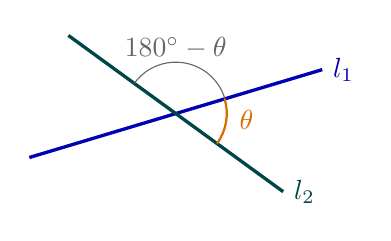
\begin{tikzpicture}[scale=0.62]
  \draw[blue!70!black, very thick] (-3,-0.9) -- (3,0.9) node[right] {$l_1$};
  \draw[teal!55!black, very thick] (-2.2,1.6) -- (2.2,-1.6) node[right] {$l_2$};
  \draw[orange!85!black, thick] (1.0,0.3) arc (16.7:-36:1.045);
  \node[orange!85!black] at (1.45,-0.13) {$\theta$};
  \draw[black!60] (-0.85,0.62) arc (144:16.7:1.05);
  \node[black!60] at (0,1.35) {$180^{\circ}-\theta$};
\end{tikzpicture}\\[1mm]
{\small Two crossing lines make two angles, $\theta$ and $180^{\circ}-\theta$. The modulus picks the acute one.}
\end{minipage}

% EXAMPLE: new; (a) uses the two lines of his 4.7 example
\begin{example}[label=ex:4.11]
Find the acute angle between
\begin{enumerate}[(a)]
  \item $l_1:\ \mathbf{r} = \col{1}{2}{3} + \lambda\col{3}{0}{-1}$ and $l_2:\ \mathbf{r} = \col{3}{-2}{-1} + \mu\col{2}{2}{1}$,
  \item $\mathbf{r} = \lambda\col{1}{2}{2}$ and $\mathbf{r} = \col{1}{0}{0} + \mu\col{-2}{1}{-2}$.
\end{enumerate}
\end{example}
\solution{
(a)\quad $\cos\theta = \dfrac{|6 + 0 - 1|}{\sqrt{10}\,\sqrt{9}} = \dfrac{5}{3\sqrt{10}}$, so $\theta = \ans{ex13411a}{58.2^{\circ}}$ (1 d.p.).

(b)\quad $\cos\theta = \dfrac{|-2 + 2 - 4|}{3\times 3} = \dfrac{4}{9}$, so $\theta = \ans{ex13411b}{63.6^{\circ}}$ (1 d.p.).
}

\begin{mistake}
\textbf{Common mistake:} dropping the modulus when the dot product is negative. In (b):
\begin{align*}
\cos\theta = \dfrac{-4}{9},\ \ \theta = 116.4^{\circ} & & \wrong \\
\cos\theta = \dfrac{|-4|}{9},\ \ \theta = 63.6^{\circ} & & \cmark
\end{align*}
$116.4^{\circ}$ is the obtuse angle between the lines. The question wants the acute one.
\end{mistake}

\begin{mistake}
\textbf{Common mistake:} using the position vectors of the lines. In (a):
\begin{align*}
\cos\theta = \dfrac{|(1,2,3)\cdot(3,-2,-1)|}{\sqrt{14}\,\sqrt{14}} = \dfrac{4}{14}, \ \ \theta = 73.4^{\circ} & & \wrong \\
\cos\theta = \dfrac{|(3,0,-1)\cdot(2,2,1)|}{\sqrt{10}\,\sqrt{9}} = \dfrac{5}{3\sqrt{10}}, \ \ \theta = 58.2^{\circ} & & \cmark
\end{align*}
\end{mistake}

% ---------------------------------------------------------------------
\clearpage
\subsection{Reflection (Line about Line)}
% ---------------------------------------------------------------------
Given two intersecting lines, we want the reflection of one line about the other. A line needs a point and a direction, so we need two points of the image line. The intersection point is one of them, because it lies on the mirror line and does not move.

\begin{definition}{Method: reflection of $l_2$ about $l_1$}
\begin{enumerate}
  \item Find the intersection $I$ of $l_1$ and $l_2$ (Section \chapnum.4.5).
  \item Take a point $A$ on $l_2$, other than $I$. Find the foot $F$ of the perpendicular from $A$ to $l_1$ (Section \chapnum.4.2).
  \item Reflect: $\overrightarrow{OA'} = 2\overrightarrow{OF} - \overrightarrow{OA}$ (Section \chapnum.4.3).
  \item The reflected line passes through $I$ with direction $\overrightarrow{IA'}$.
\end{enumerate}
\end{definition}

\begin{center}
\begin{tikzpicture}[scale=0.78]
  \draw[blue!70!black, very thick] (-0.6,0) -- (7.4,0) node[right] {$l_1$ (mirror)};
  \coordinate (I) at (6,0);
  \coordinate (A) at (1.6,-2.2);
  \coordinate (F) at (1.6,0);
  \coordinate (Ap) at (1.6,2.2);
  \draw[teal!55!black, very thick] ($(I)!1.25!(A)$) -- ($(A)!1.25!(I)$) node[above right] {$l_2$};
  \draw[orange!85!black, very thick] ($(I)!1.25!(Ap)$) -- ($(Ap)!1.25!(I)$) node[below right] {$l_3$};
  \draw[red!70!black, thick, dashed] (A) -- (Ap);
  \draw[red!70!black] (F) ++(0.22,0) -- ++(0,0.22) -- ++(-0.22,0);
  \node[pt, label=below right:{$I$}] at (I) {};
  \node[pt, label=below left:{$A$}] at (A) {};
  \node[pt, label=below left:{$F$}] at (F) {};
  \node[pt, label=above left:{$A'$}] at (Ap) {};
\end{tikzpicture}
\end{center}

\begin{caution}
The reflection of $l_2$ about $l_1$ is \textbf{not} the same as the reflection of $l_1$ about $l_2$: the mirror is the line you reflect \emph{about}. And if $l_2\parallel l_1$, there is no intersection: reflect one point of $l_2$, and keep the same direction.
\end{caution}

% EXAMPLE: from Maximus's notes, 4.7 Example 1. His COMPLETED copy has no
% handwritten working for this page; solved here by his 4.2/4.3 method,
% agreeing with his typed answer.
\begin{example}[label=ex:4.12]
Find the reflection of $l_2$ about $l_1$, where
\[
l_1:\ \mathbf{r} = \col{1}{2}{3} + \lambda\col{3}{0}{-1},\ \lambda\in\RR, \qquad
l_2:\ \mathbf{r} = \col{3}{-2}{-1} + \mu\col{2}{2}{1},\ \mu\in\RR.
\]
\end{example}
\solution{
\textbf{Step 1: intersection.} $\col{1+3\lambda}{2}{3-\lambda} = \col{3+2\mu}{-2+2\mu}{-1+\mu}$. The $y$-row gives $\mu = 2$, the $z$-row then gives $\lambda = 2$, and the $x$-row checks: $7 = 7$. So $I$ is $\ans{ex13412I}{\col{7}{2}{1}}$.

\textbf{Step 2: a point on $l_2$ and its foot.} $\mu = 0$ gives $A(3,-2,-1)$ on $l_2$. Its foot on $l_1$ is $F(4,2,2)$ (Example \ref{ex:4.3}).

\textbf{Step 3: reflected point.} $\overrightarrow{OA'} = 2\overrightarrow{OF} - \overrightarrow{OA} = \ans{ex13412A}{\col{5}{6}{5}}$ (Example \ref{ex:4.5}).

\textbf{Step 4: direction.} $\overrightarrow{IA'} = \col{5}{6}{5} - \col{7}{2}{1} = \col{-2}{4}{4} = 2\col{-1}{2}{2}$. The reflected line is
\[
l_3:\ \mathbf{r} = \col{7}{2}{1} + t\ans{ex13412d}{\col{-1}{2}{2}},\ t\in\RR.
\]
Check: $l_2$ and $l_3$ make the same angle with $l_1$, since $\dfrac{|(2,2,1)\cdot(3,0,-1)|}{3} = \dfrac{|(-1,2,2)\cdot(3,0,-1)|}{3} = \dfrac{5}{3}$.
}

\begin{mistake}
\textbf{Common mistake:} using the foot $F$ instead of the reflected point $A'$ for the direction.
\begin{align*}
\overrightarrow{IF} = \col{4}{2}{2} - \col{7}{2}{1} = \col{-3}{0}{1},\ \ l_3:\ \mathbf{r} = \col{7}{2}{1} + t\col{-3}{0}{1} & & \wrong \\
\overrightarrow{IA'} = \col{5}{6}{5} - \col{7}{2}{1} = 2\col{-1}{2}{2},\ \ l_3:\ \mathbf{r} = \col{7}{2}{1} + t\col{-1}{2}{2} & & \cmark
\end{align*}
$F$ lies on the mirror, so $\overrightarrow{IF}$ is parallel to $l_1$: the ``answer'' is $l_1$ itself.
\end{mistake}


